% documentclass
% set font size=11 (11pt)
% set paper format=A4 (a4paper)
% set equation alignment to left (fleqn)
\documentclass[11pt,a4paper,fleqn]{article}


% Preamble
% use the inputenc and fontenc packages to use French accents
\usepackage[utf8]{inputenc}
\usepackage[T1]{fontenc}
% for matrices / vectors
\usepackage{amsmath}
% allow for arbitrary font size
\usepackage{anyfontsize}
% for color
\usepackage{xcolor}
% for pseudocolor
\usepackage{algorithm,algpseudocode}
% for code samples
\usepackage{listings}
% set the font as Time New Roman (the Latex equivalent, at least)
% \usepackage{mathptmx}
% set the size of the document margins using the geometry package
\usepackage[lmargin=0.97in,rmargin=0.97in,tmargin=1.4in,bmargin=1.4in]{geometry}
% turn the color of footnote markers to black
\renewcommand\thefootnote{\textcolor{black}{\arabic{footnote}}}
% suppress indents on footnotes
\usepackage[hang,flushmargin]{footmisc}
% automatically generates colored brackets around references
\usepackage{fncylab} \labelformat{equation}{(#1)}
% supress indent on new paragraphs
\setlength{\parindent}{0pt}
% use the amsmath package to include mathematical symbols
\usepackage{amsmath}
% suppress the space between the left margin and the equations (fleqn still leaves some space by default)
\setlength{\mathindent}{0pt}
% create a new environment to left flush the equation with the align environment
\makeatletter
\newenvironment{lflalign}{ \vspace{-3mm}%
  \def\align@preamble{%
    &\strut@
    \setboxz@h{\@lign$\m@th\displaystyle{####}$}%
    \ifmeasuring@\savefieldlength@\fi
    \set@field
    \hfil
    \tabskip\z@skip
    &\setboxz@h{\@lign$\m@th\displaystyle{{}####}$}%
    \ifmeasuring@\savefieldlength@\fi
    \set@field
    \hfil
    \tabskip\alignsep@
  }
  \flalign}
{\endflalign}
\makeatother
% use the ammssymb package to use mathematical symbols
\usepackage{amssymb}
% create new commands for mathematical symbols
\DeclareMathOperator{\N}{\mathbb{N}}
\DeclareMathOperator{\Z}{\mathbb{Z}}
\DeclareMathOperator{\Q}{\mathbb{Q}}
\DeclareMathOperator{\R}{\mathbb{R}}
\DeclareMathOperator{\Pb}{\mathbb{P}}
% declare the cmsy (computer modern symbol) math alphabet to define appropriate fonts for the U and N mathematical symbols
\DeclareMathAlphabet\mathbcal{OMS}{cmsy}{m}{n}
% create new commands for mathematical symbols
\DeclareMathOperator{\E}{\mathbcal{E}}
\DeclareMathOperator{\Ex}{\mathbb{E}}
\DeclareMathOperator{\F}{\mathbcal{F}}
\DeclareMathOperator{\G}{\mathbcal{G}}
\DeclareMathOperator{\M}{\mathbcal{M}}
\DeclareMathOperator{\HH}{\mathbcal{H}}
\DeclareMathOperator{\QQ}{\mathbcal{Q}}
\DeclareMathOperator{\PP}{\mathbcal{P}}
\DeclareMathOperator{\Noo}{\mathbcal{N}}
\DeclareMathOperator{\U}{\mathbcal{U}}
% use the bbm package to be able to use the double stroke 1 for the indicator function
\usepackage{bbm}
\DeclareMathOperator{\ind}{\mathbbmss{1}}
% use the bm package to use bold characters in math mode
\usepackage{bm}
% create a new command for black square bullets
\newcommand{\bs}{\scalebox{0.7}{$\blacksquare$} \hspace{2mm}}
% use the relsize package to be abe to change the size of mathematical symbols
\usepackage{relsize}
% define a new command for in-line small summation
\newcommand{\ssumm}[2]{\underset{\scriptscriptstyle #1}{\overset{\scriptscriptstyle #2}{\mathlarger{\mathlarger{\mathlarger{\Sigma}}}}} \hspace{0.5mm}}
% define a new command for in-line small products
\newcommand{\sprod}[2]{\underset{\scriptscriptstyle #1}{\overset{\scriptscriptstyle #2}{\mathlarger{\mathlarger{\mathlarger{\Pi}}}}} \hspace{0.5mm}}
% Use the caption package to customize captions (titles) of tables and graphs
\usepackage[font=small,labelfont=bf]{caption}
% use float package to force figure the be positioned where indicated
\usepackage{float}
% use the graphicx package to be able to resize tables
\usepackage{graphicx}

\begin{document}

% command to check unused bibliography entries
% \nocite{*}

\textbf{HMM - TP noté à rendre pour le 07/04/2020 - Gaël Savouré}

\vspace{5mm}

\textbf{I. Chaînes de Markov}

\vspace{5mm}
\textit{I.2.a Matrice de transitions}

\vspace{5mm}
\textcolor{orange}{A quelles probabilités correspond la première ligne de la matrice de transition ? et celles de la
dernière colonne ?}

La première ligne correspond aux probabilités d'avoir chaque lettre de l'alphabet en début de mot.

La dernière colonne correspond, pour chaque lettre, aux probabilités de terminer le mot.

\vspace{5mm}
\textcolor{orange}{Pour chaque lettre de l’alphabet, indiquer la transition la plus fréquente depuis cette lettre.}

\lstset{language=Python}
\lstset{frame=lines}
\lstset{caption={Output - Transitions les plus fréquentes}}
\lstset{label={lst:code_direct}}
\lstset{basicstyle=\footnotesize}
\begin{lstlisting}
Most frequent transitions:
letter ' ': --> 't' (proba = 0.16452225)
letter 'a': --> 'n' (proba = 0.22051689)
letter 'b': --> 'e' (proba = 0.28275808)
letter 'c': --> 'o' (proba = 0.16686338)
letter 'd': --> ' ' (proba = 0.59884373)
letter 'e': --> ' ' (proba = 0.36047379)
letter 'f': --> ' ' (proba = 0.39653963)
letter 'g': --> ' ' (proba = 0.31566736)
letter 'h': --> 'e' (proba = 0.46971451)
letter 'i': --> 'n' (proba = 0.24528243)
letter 'j': --> 'o' (proba = 0.46979866)
letter 'k': --> ' ' (proba = 0.37225637)
letter 'l': --> 'e' (proba = 0.17086033)
letter 'm': --> 'e' (proba = 0.26768727)
letter 'n': --> ' ' (proba = 0.29421872)
letter 'o': --> 'n' (proba = 0.16035077)
letter 'p': --> 'e' (proba = 0.19473793)
letter 'q': --> 'u' (proba = 0.96368715)
letter 'r': --> 'e' (proba = 0.24477159)
letter 's': --> ' ' (proba = 0.43030156)
letter 't': --> 'h' (proba = 0.33937505)
letter 'u': --> 'r' (proba = 0.15036937)
letter 'v': --> 'e' (proba = 0.61843409)
letter 'w': --> 'a' (proba = 0.20323878)
letter 'x': --> 't' (proba = 0.20061728)
letter 'y': --> ' ' (proba = 0.77582944)
letter 'z': --> 'e' (proba = 0.55662188)
letter ' ': --> ' ' (proba = 1.0)
\end{lstlisting}

\textit{I.2.a Générer un mot}

\vspace{5mm}
\textcolor{orange}{Ecrire une fonction etat\_suivant qui génère un état (à t+1) à partir de l’état courant (à t) et à
l’aide de la matrice de transitions et de la fonction de répartition.}

\lstset{language=Python}
\lstset{frame=lines}
\lstset{caption={Fonction etat\_suivant}}
\lstset{label={lst:code_direct}}
\lstset{basicstyle=\footnotesize}
\begin{lstlisting}
def nextState(transition_matrix, dic, state):
    proba_state = transition_matrix[int(state)-1]
    next_state = np.random.choice(list(dic.keys()), p=proba_state)
    return proba_state, str(next_state)
\end{lstlisting}

\vspace{5mm}
\textcolor{orange}{Afficher sur un graphique la fonction de répartition pour une ligne de la matrice de transition
et expliquer son rôle pour la génération de l’état à t+1.}

\begin{center}
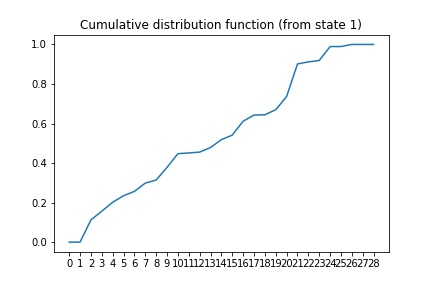
\includegraphics[scale = 0.5]{cdf_state_1.jpg}
\end{center}

La fonction de répartition sert à la génération de l'état t+1 car plus un segment est pentu entre deux état, plus la probabilité de transition vers cet état est forte. On voit bien depuis cette fonction de répartition que transiter vers la lettre 't' (état 21) depuis le début d'un mot (état 1) a la probabilité la plus forte.

\vspace{5mm}
\textcolor{orange}{Utiliser cette fonction pour écrire la fonction genere\_state\_seq qui génère une séquence d’états jusqu’à aboutir à l’état final (28).}

\lstset{language=Python}
\lstset{frame=lines}
\lstset{caption={Fonction genere\_state}}
\lstset{label={lst:code_direct}}
\lstset{basicstyle=\footnotesize}
\begin{lstlisting}
def genere_state_seq(transition_matrix, dic, final_state):
    generated_states = []
    state = '1'
    while(state != final_state):
        _, state = nextState(transition_matrix, dic, state)
        generated_states.append(state)
    return generated_states
\end{lstlisting}

\vspace{5mm}
\textcolor{orange}{Ecrire une fonction display\_seq qui transforme une séquence d’états en séquence de caractères, à l’aide d’un dictionnaire.}

\lstset{language=Python}
\lstset{frame=lines}
\lstset{caption={Fonction display\_seq}}
\lstset{label={lst:code_direct}}
\lstset{basicstyle=\footnotesize}
\begin{lstlisting}
def display_seq(dic, states):
    elements = []
    for state in states:
        elements.append(dic[state])
    return ''.join(elements)
\end{lstlisting}

\vspace{5mm}
\textcolor{orange}{Utiliser ces fonctions pour générer des mots et donner des exemples de mots générés.}

\lstset{language=Python}
\lstset{frame=lines}
\lstset{caption={Output - Génération de mots}}
\lstset{label={lst:code_direct}}
\lstset{basicstyle=\footnotesize}
\begin{lstlisting}
mby 
w 
so 
tlt 
teay 
\end{lstlisting}

\vspace{5mm}
\textit{I.2.c Générer une phrase}

\textcolor{orange}{On veut générer une suite de mots (phrase). Créer un état final de phrase (état 29,
correspondant au caractère . ) dont la probabilité de transition vers cet état depuis un état
final de mot est 0.1. Ecrire une fonction modifie\_mat\_dic qui modifie la matrice de transition
et le dictionnaire en conséquence.}

\lstset{language=Python}
\lstset{frame=lines}
\lstset{caption={Fonction modifie\_mat\_dic}}
\lstset{label={lst:code_direct}}
\lstset{basicstyle=\footnotesize}
\begin{lstlisting}
def modifyMatAndDic(transition_matrix, dic):
    dic_2 = dic.copy()

    # modify dic
    dic_2['28'] = '' # since P(28 -> 1) = 0.9
    dic_2['29'] = '.'

    # add row
    transition_matrix_2 = np.vstack((transition_matrix, np.zeros((1,28))))

    # add column
    transition_matrix_2 = np.hstack((transition_matrix_2, np.zeros((29,1))))

    # add probabilities
    transition_matrix_2[27,0]=0.9 # probability to go from final state '' to beginning of word ' '
    transition_matrix_2[27,28]=0.1 # probability to go from end of word to dot '.'
    transition_matrix_2[27,27]=0.0
    transition_matrix_2[28,28]=1.0

    return transition_matrix_2, dic_2
\end{lstlisting}

\vspace{5mm}
\textcolor{orange}{Donner des exemples de phrases générées.}

\lstset{language=Python}
\lstset{frame=lines}
\lstset{caption={Output - phrases générées}}
\lstset{label={lst:code_direct}}
\lstset{basicstyle=\footnotesize}
\begin{lstlisting}
ganoum buccovaprerined ichithe istoprgavinthe warave g re ankitig ilo er ot are pthonecad cud als.
w e ppathe to spe oulee darhie cryorthag.
spre aravey bitr tisathege cher gne worone an cein achans of.
ulvedevethe morthe bley f bund he cre thigons we thes wheviftitanoretes tw orly d coper benobole tiatang.
on weaigweacokeioves ten hatheroras at ined th musid of nedsucore heg.
\end{lstlisting}

\vspace{5mm}
\textit{I.3. Reconnaissance de la langue}

\vspace{5mm}
\textcolor{orange}{Ecrire une fonction calc\_vraisemblance qui calcule la vraisemblance du modèle français pour une phrase donnée en multipliant les probabilités de transition.}

\lstset{language=Python}
\lstset{frame=lines}
\lstset{caption={Fonction vraisemblance}}
\lstset{label={lst:code_direct}}
\lstset{basicstyle=\footnotesize}
\begin{lstlisting}
def computeLikelihood(sentence, transition_matrix):
    new_sentence = processSentence(sentence) # transfrom sentences with + and -
    state_prev = '1'
    proba_list = []
    for letter in new_sentence[1:]:
        if letter == '-':
            state = '1'
        elif letter == '+':
            state = '28'
        else:
            state = dic_inv[letter]
        proba = transition_matrix[int(state_prev)-1, int(state)-1]
        proba_list.append(proba)
        state_prev = state
    return proba_list
\end{lstlisting}

\vspace{5mm}
\textcolor{orange}{Calculer la vraisemblance des modèles français et anglais pour la phrase « to be or not to be ».}

\lstset{language=Python}
\lstset{frame=lines}
\lstset{caption={Output - Vraisemblance "to be or not to be."}}
\lstset{label={lst:code_direct}}
\lstset{basicstyle=\footnotesize}
\begin{lstlisting}
***** to be or not to be *****
likelihood (fr): 5.96020810186864e-29
likelihood (en): 8.112892227809414e-19
\end{lstlisting}

\vspace{5mm}
On remarque que la vraisemblance est plus forte en utilisant le modèle anglais.

\vspace{5mm}
\textcolor{orange}{De même calculer la vraisemblance des modèles français et anglais pour la phrase « etre ou ne
pas etre ».}

\lstset{language=Python}
\lstset{frame=lines}
\lstset{caption={Output - Vraisemblance "etre ou ne pas etre."}}
\lstset{label={lst:code_direct}}
\lstset{basicstyle=\footnotesize}
\begin{lstlisting}
***** etre ou ne pas etre *****
likelihood (fr): 1.145706887234789e-18
likelihood (en): 4.462288711775253e-23
\end{lstlisting}

\vspace{5mm}
On remarque que la vraisemblance est plus forte en utilisant le modèle français.

\vspace{5mm}
\textbf{II. HMM}
\vspace{5mm}

\textit{II. 2. Génération de séquences d’observations}

\vspace{5mm}
\textcolor{orange}{A quoi correspondent les zéros de la matrice B ? et ceux de la matrice A et du vecteur ?}

La matrice B contient les probabilités d'observations depuis les différents états. Un zéro situé aux coordonnées (i,j) signifie qu'il est impossible d'obtenir l'observation (i+1) depuis l'état caché (j+1).

La matrice A contient les probabilités de transition entre les différents états cachés. Un zéro situé aux coordonnées (i,j) signifie qu'il est impossible de transiter de l'état (i+1) à (j+1).

Le vecteur $pi$ contient les probabilités associées aux états initiaux. Un zéro situé à la composante i signifie qu'il est impossible de commencer par l'état (i+1).

\vspace{5mm}
\textcolor{orange}{Ecrire une fonction etat\_suivant qui génère un état $q_{t+1}$ à partir de l’état courant $q_t$ à l’aide de la matrice de transitions et de la fonction de répartition cumsum.}

\lstset{language=Python}
\lstset{frame=lines}
\lstset{caption={Fonction etat\_suivant}}
\lstset{label={lst:code_direct}}
\lstset{basicstyle=\footnotesize}
\begin{lstlisting}
def nextState(transition_matrix, state):
    proba_state = transition_matrix[state-1]
    proba_cum = np.cumsum(proba_state)
    n = np.random.random()
    next_state = len(np.where(proba_cum < n)[0])+1
    return next_state, proba_cum
\end{lstlisting}

\vspace{5mm}
\textcolor{orange}{Afficher la fonction de répartition pour une ligne de la matrice de transition et expliquer son rôle pour la génération de l’état à t+1.}

\begin{center}
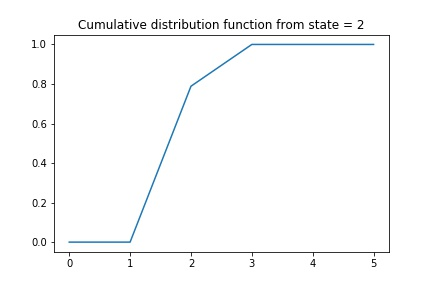
\includegraphics[scale = 0.5]{cdf_part_2.jpeg}
\end{center}

La fonction de répartition sert à la génération de l'état t+1 car plus un segment est pentu entre deux état, plus la probabilité de transition vers cet état est forte. On voit depuis cette fonction de répartition que transiter vers l'état 2 depuis l'état 2 est la transition avec la plus forte probabilité.

\vspace{5mm}
\textcolor{orange}{Générer une séquence d’observations suivant le modèle de Markov Caché du chiffre 0. On commencera par générer une séquence d’états suivant ce modèle à l’aide de la fonction etat\_suivant. Puis on générera la séquence d’observations par le même procédé.}

\lstset{language=Python}
\lstset{frame=lines}
\lstset{caption={Fonctions pour générer des observations}}
\lstset{label={lst:code_direct}}
\lstset{basicstyle=\footnotesize}
\begin{lstlisting}
def generateStates(initial_matrix, transition_matrix):
    state_prev = np.where(np.max(initial_matrix))[0][0]+1
    state_sq = []
    for i in range(v.shape[1]):
        state_sq.append(state_prev)
        state, _ = nextState(transition_matrix, state_prev)
        state_prev = state
    return state_sq

def observationsFromStates(observation_matrix, state_sq):
    observation_sq = []
    for state in state_sq:
        proba_observation = observation_matrix[:,state-1]
        proba_cum = np.cumsum(proba_observation)
        n = np.random.random()
        observation = len(np.where(proba_cum < n)[0])+1
        observation_sq.append(observation)
    return observation_sq
\end{lstlisting}

\vspace{5mm}
\textcolor{orange}{Visualiser le résultat sous forme d’image. Générer des séquences pour le chiffre 7 et le
chiffre 1 (matrices B1.txt, B7.txt, etc...)}

\begin{center}
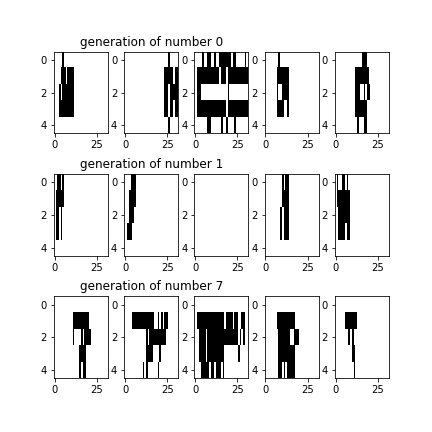
\includegraphics[scale = 0.5]{number_generation.jpg}
\end{center}

\vspace{5mm}
\textit{II.3. Calcul de la vraisemblance de séquences d’observations}

\vspace{5mm}
\textcolor{orange}{Calculer la vraisemblance de ces séquences suivant chacun des modèles (0, 1 et 7) par l’algorithme de Viterbi (on pourra implémenter la version logarithmique de cet algorithme). Pour cela les matrices A, B et $\pi$ seront converties en logarithmes (utiliser np.log).}

\lstset{language=Python}
\lstset{frame=lines}
\lstset{caption={Algorithme de Viterbi}}
\lstset{label={lst:code_direct}}
\lstset{basicstyle=\footnotesize}
\begin{lstlisting}
def likelihoodViterbi(seq, A, B, pi):

    A = np.ma.log(A).filled(-500)
    B = np.ma.log(B).filled(-500)
    pi = np.ma.log(pi).filled(-500)

    vit_matrix = np.zeros((A.shape[0], len(seq)))
    # initialization
    for state in range(1,vit_matrix.shape[0]+1):
        observation = seq[0]
        proba_start = pi[state-1]
        proba_obs = B[state-1,observation-1]
        vit_matrix[state-1,0] = proba_start + proba_obs
    # fill the rest of the matrix
    state_list = np.arange(vit_matrix.shape[0])+1
    for obs_idx in range(len(seq[1:])):
        observation = seq[obs_idx]
        for state in state_list:
            proba_trajectories = []
            for state_prev in state_list:
                delta_prev = vit_matrix[state_prev-1,obs_idx]
                proba_obs = B[observation-1,state-1]
                proba_state = A[state_prev-1,state-1]
                proba_trajectories.append(delta_prev + proba_obs + proba_state)
            vit_matrix[state-1,obs_idx+1] = np.max(proba_trajectories)
    return np.max(vit_matrix[:,-1])
\end{lstlisting}

\vspace{5mm}
\textcolor{orange}{II.3.2 Donner le résultat de la classification des images de test en considérant un problème à trois classes : 0, 1 et 7.}

\lstset{language=Python}
\lstset{frame=lines}
\lstset{caption={Output - Résultats de classification (SeqTest0.txt)}}
\lstset{label={lst:code_direct}}
\lstset{basicstyle=\footnotesize}
\begin{lstlisting}
Sequence 1: model prediction 0
Sequence 2: model prediction 0
Sequence 3: model prediction 0
Sequence 4: model prediction 0
Sequence 5: model prediction 0
Sequence 6: model prediction 0
Sequence 7: model prediction 0
Sequence 8: model prediction 0
Sequence 9: model prediction 0
Sequence 10: model prediction 0
\end{lstlisting}


\lstset{language=Python}
\lstset{frame=lines}
\lstset{caption={Output - Résultats de classification (SeqTest1.txt)}}
\lstset{label={lst:code_direct}}
\lstset{basicstyle=\footnotesize}
\begin{lstlisting}
Sequence 1: model prediction 1
Sequence 2: model prediction 1
Sequence 3: model prediction 1
Sequence 4: model prediction 1
Sequence 5: model prediction 1
Sequence 6: model prediction 1
Sequence 7: model prediction 1
Sequence 8: model prediction 1
Sequence 9: model prediction 1
Sequence 10: model prediction 1
\end{lstlisting}

\lstset{language=Python}
\lstset{frame=lines}
\lstset{caption={Output - Résultats de classification (SeqTest7.txt)}}
\lstset{label={lst:code_direct}}
\lstset{basicstyle=\footnotesize}
\begin{lstlisting}
Sequence 1: model prediction 7
Sequence 2: model prediction 7
Sequence 3: model prediction 1
Sequence 4: model prediction 7
Sequence 5: model prediction 7
Sequence 6: model prediction 7
Sequence 7: model prediction 7
Sequence 8: model prediction 7
Sequence 9: model prediction 7
Sequence 10: model prediction 7
\end{lstlisting}

\end{document}